\documentclass[../main.tex]{subfiles}
\graphicspath{{\subfix{../images/}}}
\begin{document}
	
	\chapter{Photodetectors and their characterization}\label{chap:theory}
	\section{Charged-coupled devices (CCDs)}\label{sect:CCD}
	The detector that will be flown on the satellite is a photo-sensitive detector, called a charged-coupled device (CCD). An image of a CCD can be seen in figure \ref{fig:CCDchip}. Before we may describe the characterization procedure, we need to understand how the detector works. This section will outline the basic physics of the CCD detector, following the treatment given in chapter 7 of \cite{solidstatephysicsbook}.
	
	\begin{figure}[h!]
		\centering
		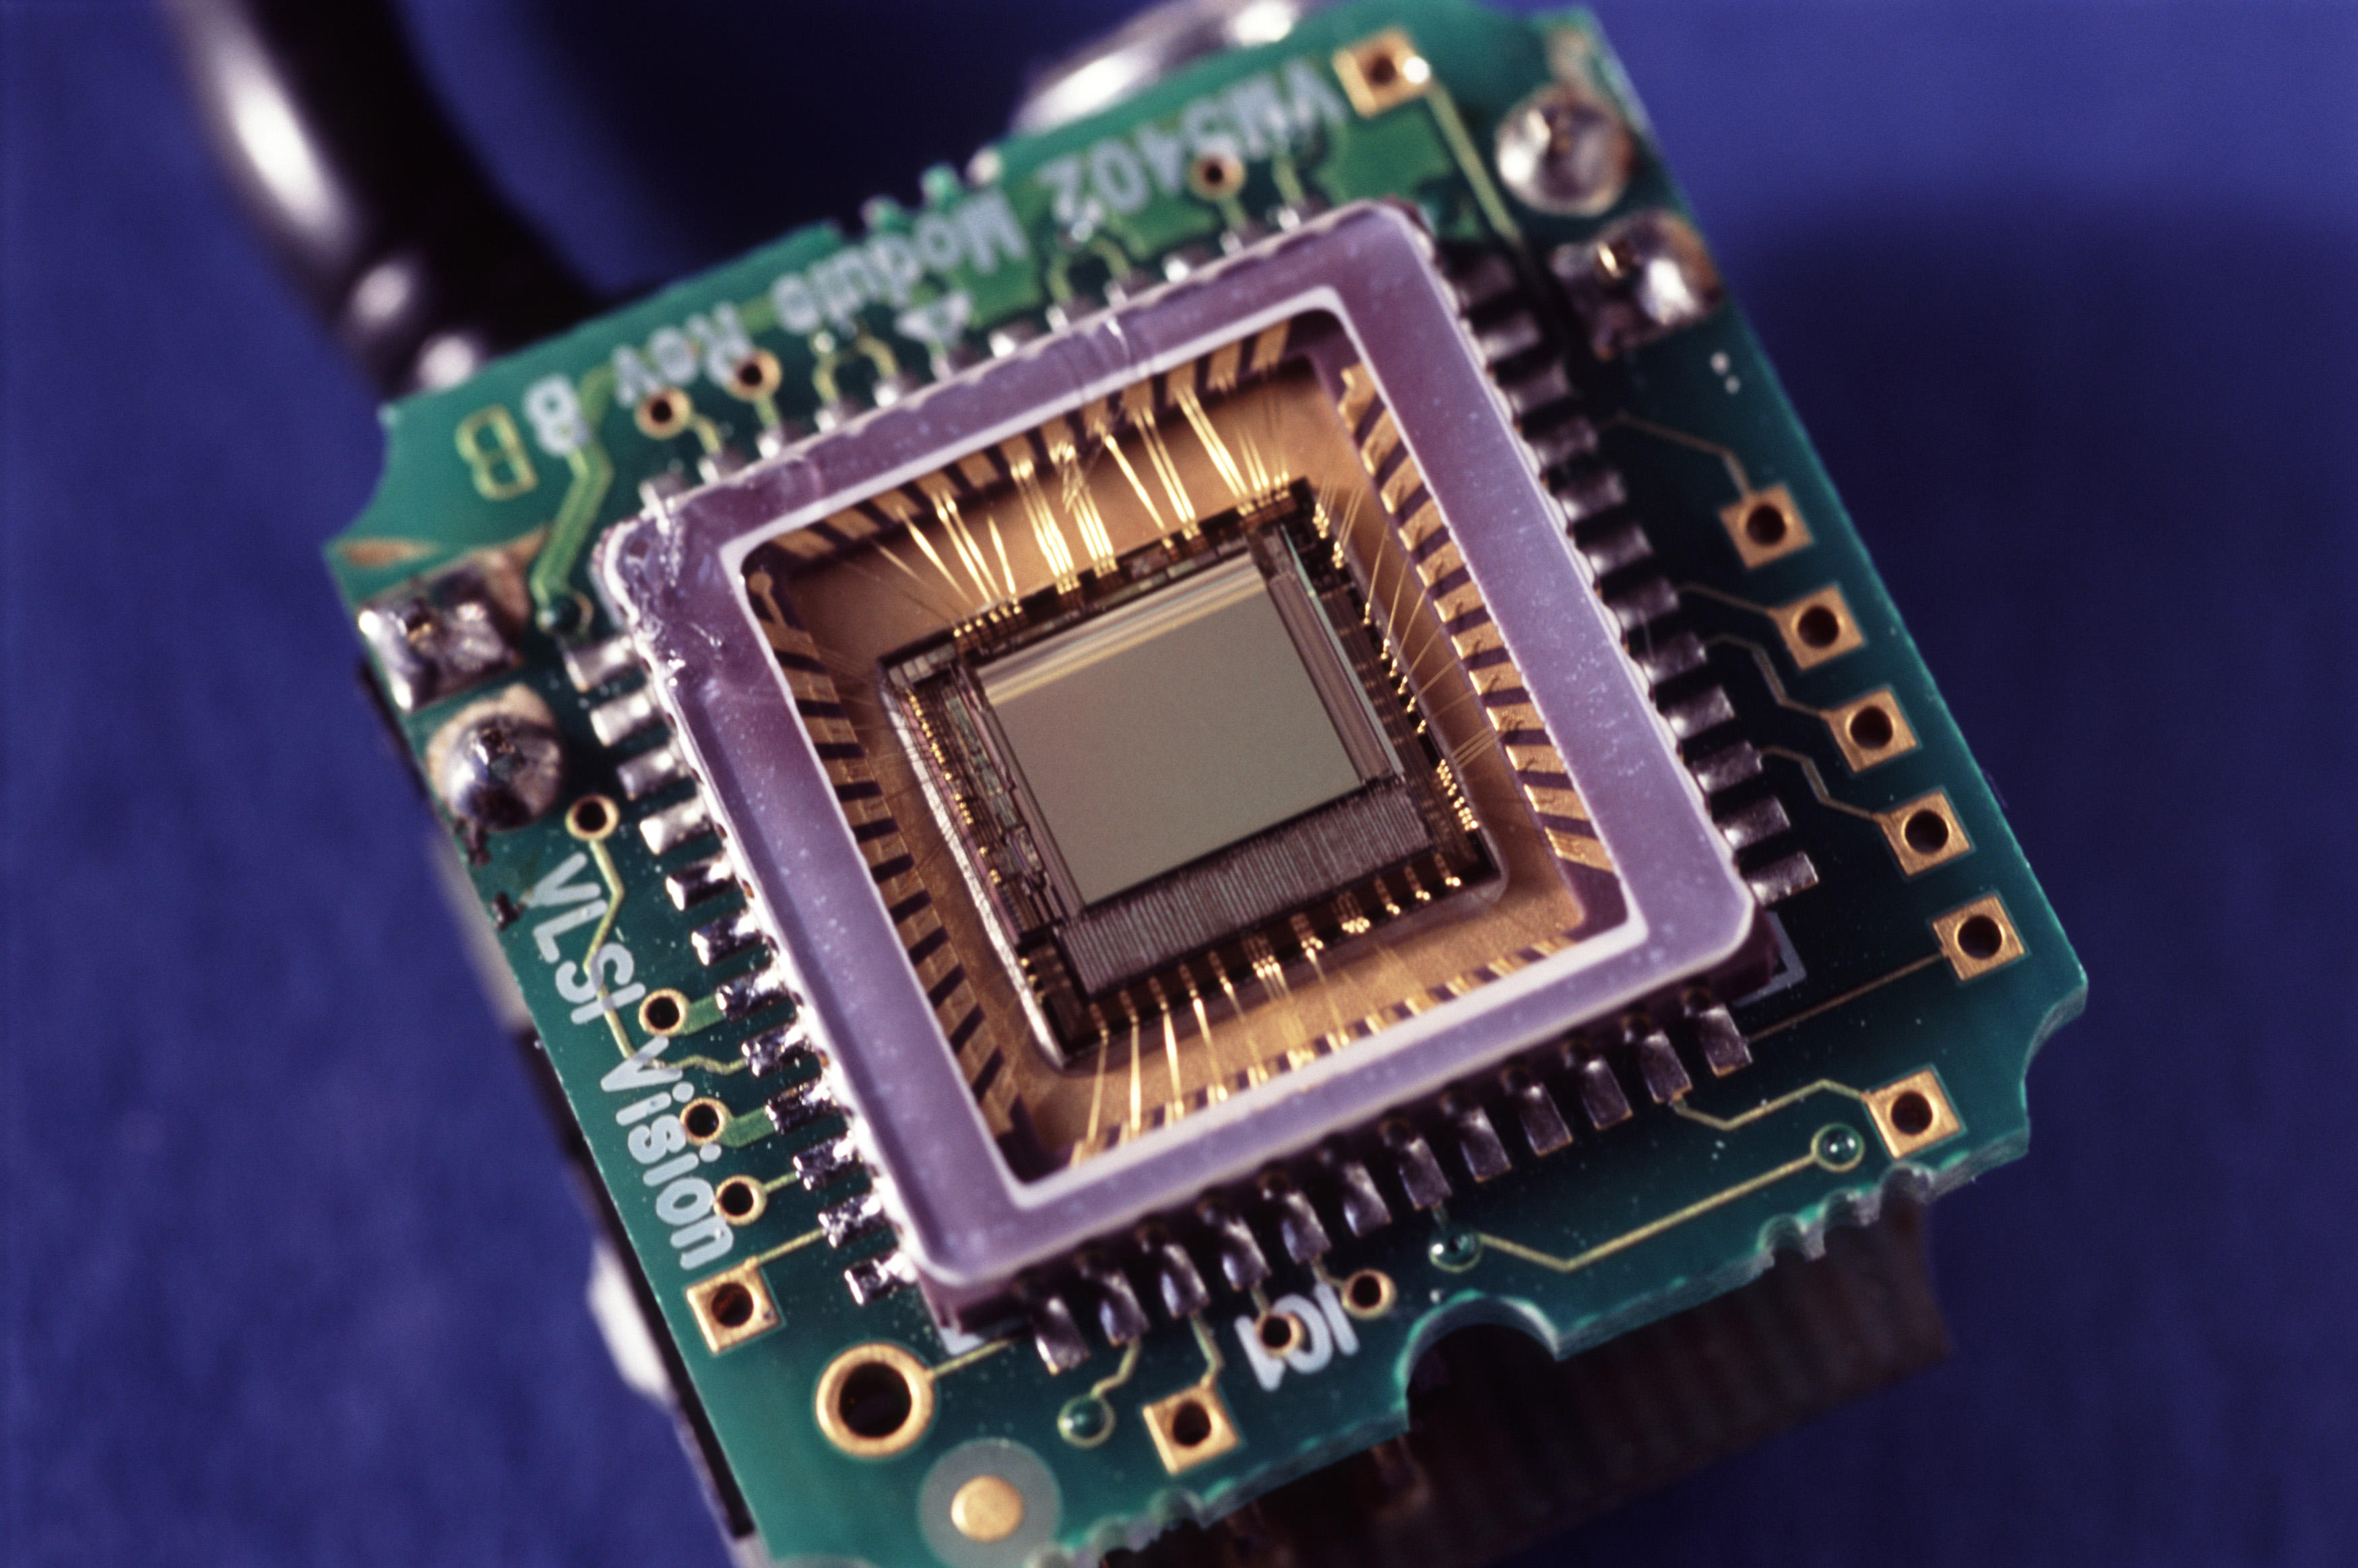
\includegraphics[width=1\textwidth]{ccd_sensor.jpg}
		\caption{Macro image of a CCD chip. By  \url{http://sciencestockphotos.com/free/electrical/slides/ccd_sensor.html}, Accessed December 13th, CC 4.0.}
		\label{fig:CCDchip}
	\end{figure}
	
	A CCD is a solid-state image sensor used to detect light. It is an integrated circuit that is essentially an array of metal-oxide-semiconductor (MOS) capacitors (MOSCAP) \cite{IEEMOS} forming a photoactive region of silicon. Each of these MOSCAPs represents a pixel in the image. Understanding how the pixels work relies on a solid understanding of the semi-conductor which is described first. A thorough discussion of the physics enables a true appreciation of the effects of the detector. We may then describe the MOSCAP, which relies on the working principles of the pn-junction. To conclude, the readout of charge, which is what in the end will be interpreted as the image, is described.
	
	\subsection{Semiconductors}
	The photoactive\footnote{A photoactive region is a solid state material that interacts with light trough the photoelectric effect.} region of the CCD, is an epitaxial\footnote{An epitaxial layer refers to a growth on top of a crystal or other material.} layer of silicon \cite{comphistmus}. Silicon is a semiconductor, which is a kind of solid-state material that has several useful properties when designing a detector. In order to understand the pixel of the CCD, we need to understand the interaction of light with the solid-state material. 
	
	A semiconductor is a type of solid-state material, which is neither a conductor nor an insulator\cite{solidstatephysicsbook}. This distinction between insulators and conductors is defined from the difference in the density of states at the chemical potential at a temperature of $0K$\cite{solidstatephysicsbook}. For metals, we have a finite density of states, see figure \ref{fig:bands}. Otherwise, it is an insulator or a semiconductor. Solid state materials have bands representing a range of available energy states of the electrons that make up the solid. The absence of bands, the separation between two bands, is called a bandgap. This gap is usually in the order of magnitude of a few electron volts. A semiconductor is defined as a material for which the bandgap between the highest occupied states in the valence band, and the lowest unoccupied states in the conduction band, is sufficiently small, enabling thermal excitation of electrons across the gap. The valence and conduction bands lie on either side of the fermi energy, the valence band being below \cite{solidstatephysicsbook}. The band structures of different materials are depicted in figure \ref{fig:bands}.
	
	\begin{figure}[h!]
		\centering
		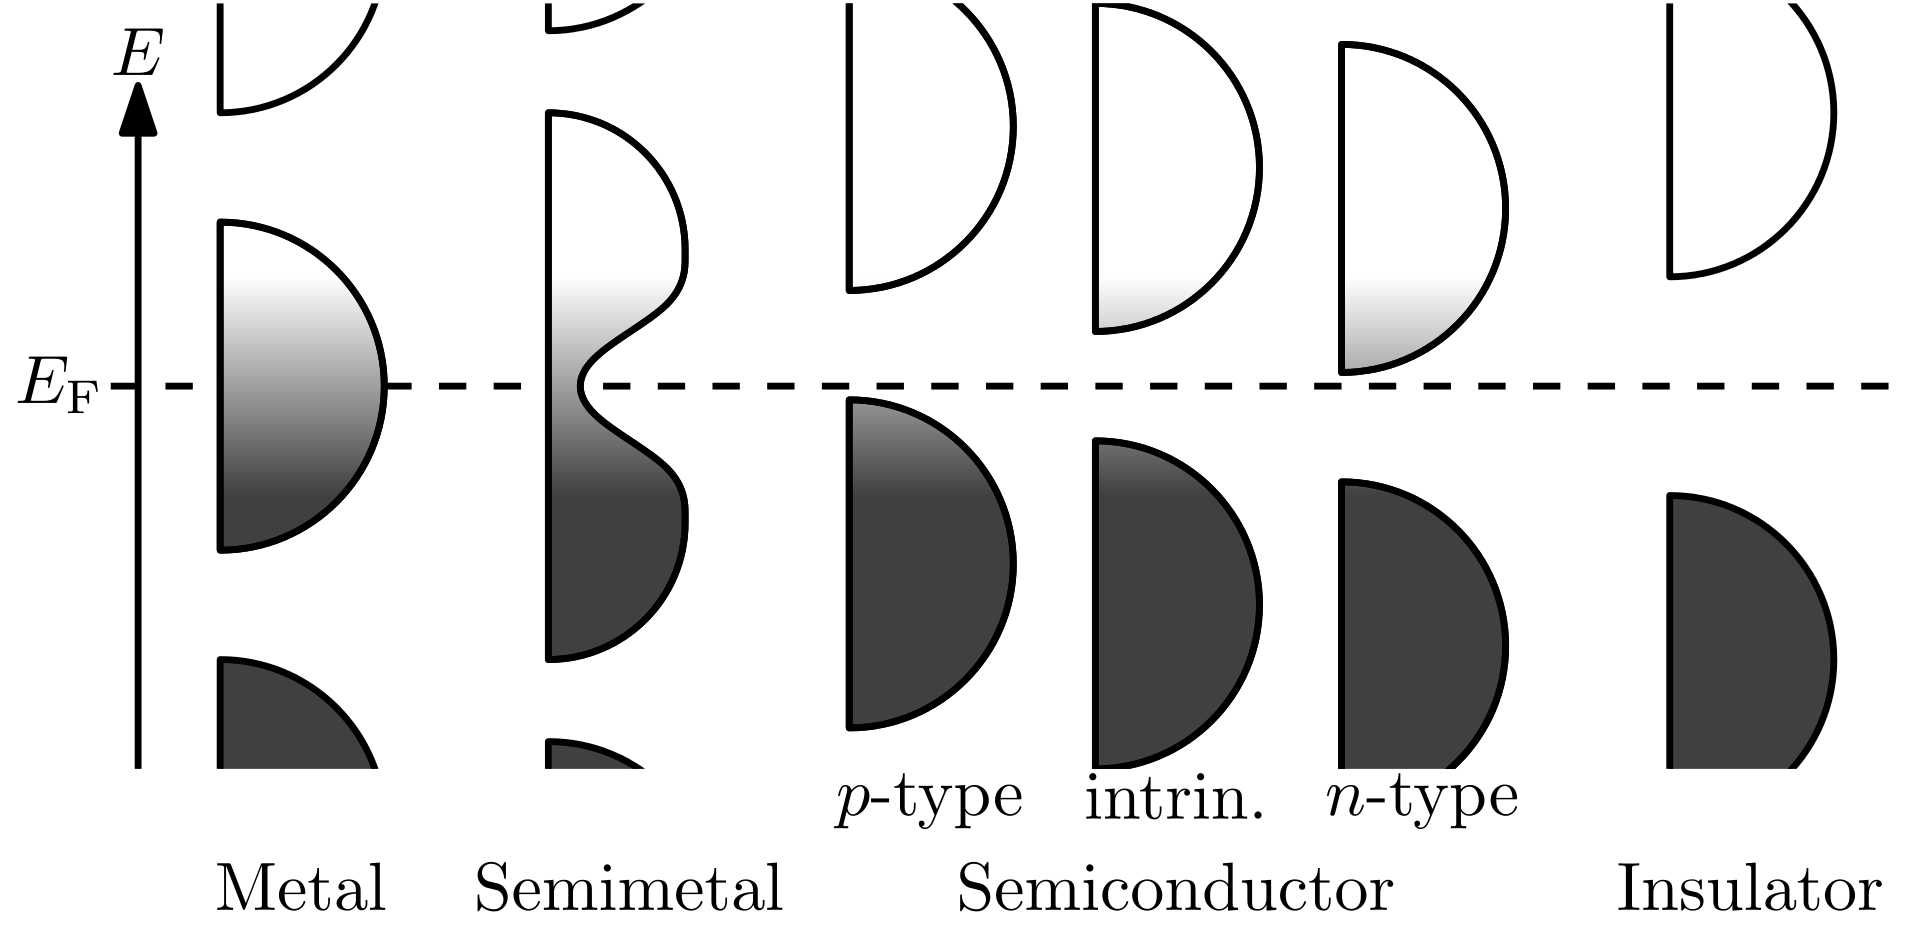
\includegraphics[width=0.7\textwidth]{Band_filling_diagram.png}
		\caption{Electronic states in various types of materials. Along the first axis is the density of states, while the second denotes the energy of the state. Shading is the Fermi–Dirac distribution with black denoting all states filled, and white none. By Nanite - Own work, CC0, https://commons.wikimedia.org/w/index.php?curid=26707196}
		\label{fig:bands}
	\end{figure}
	
	A semiconductor is a solid, for which the chemical potential at absolute zero is placed at an energy level such that the density of states is zero \cite{solidstatephysicsbook}. This is around the center of the bandgap. At finite temperature, some of the electrons from the valence band are thermally excited into the conduction band. This leaves behind so-called holes in the valence band. Holes are simply a convenient way to describe the absence of electrons, allowing us to treat them as positively charged quasiparticles\footnote{A quasiparticle is a phenomena that occurs when microscopic complicated systems behave is if they contain particles.}. The movement of electrons through the valence band is permitted by the presence of holes, which in turn can be seen as the movement of a hole in the opposite direction. Holes are hence charge carriers in the valence band allowing conduction. We call electrons and holes 'carriers', and the concentration of carriers are in part what determines the conduction properties of a material \cite{solidstatephysicsbook}.  
	
	The concentration of carriers in an intrinsic semiconductor, that is pure, is too low to give an appreciable contribution to conduction properties \cite{solidstatephysicsbook}. A way to circumvent this problem is by doping the semiconductor. This is a process in which we introduce impurities in the solid. These impurities, called dopants, can either function as donors, also called \textbf{n doping}, in which they can donate electrons to the solid, or as acceptors, also called \textbf{p doping}, in which they take electrons in turn producing a hole. N dopants are chosen such that, at not too high temperatures, the states lie just below the conduction band minimum (CBM), while the p dopant states are just above the valence band maximum (VBM). The physics of doped semiconductors is the basis of the \textbf{pn-junction} that makes up the MOSCAP.
	
	\subsection{The pn-junction} 
	The MOSCAP is an example of a practical technological application of semiconductor physics based on the working principles of the pn-junction. It is sometimes also called a diode \footnote{A diode is a kind of electrical component that acts as a valve for the current in a circuit.}. A description of this application allows us to understand how the interaction of light with the solid-state material, leads to charge generation in the pixel, which is ultimately read out and interpreted as contrast in an image. 
	
	The pn-junction is the boundary between regions of a p- and n-doped semiconductor. Such a region can be constructed by doping inhomogeneously \cite{solidstatephysicsbook}. In the n-doped region, most donors are ionized, and the majority carriers are electrons, while in the p-doped region, acceptors are negatively charged, and the majority carriers are holes. 
	\begin{figure}[h!]
		\centering
		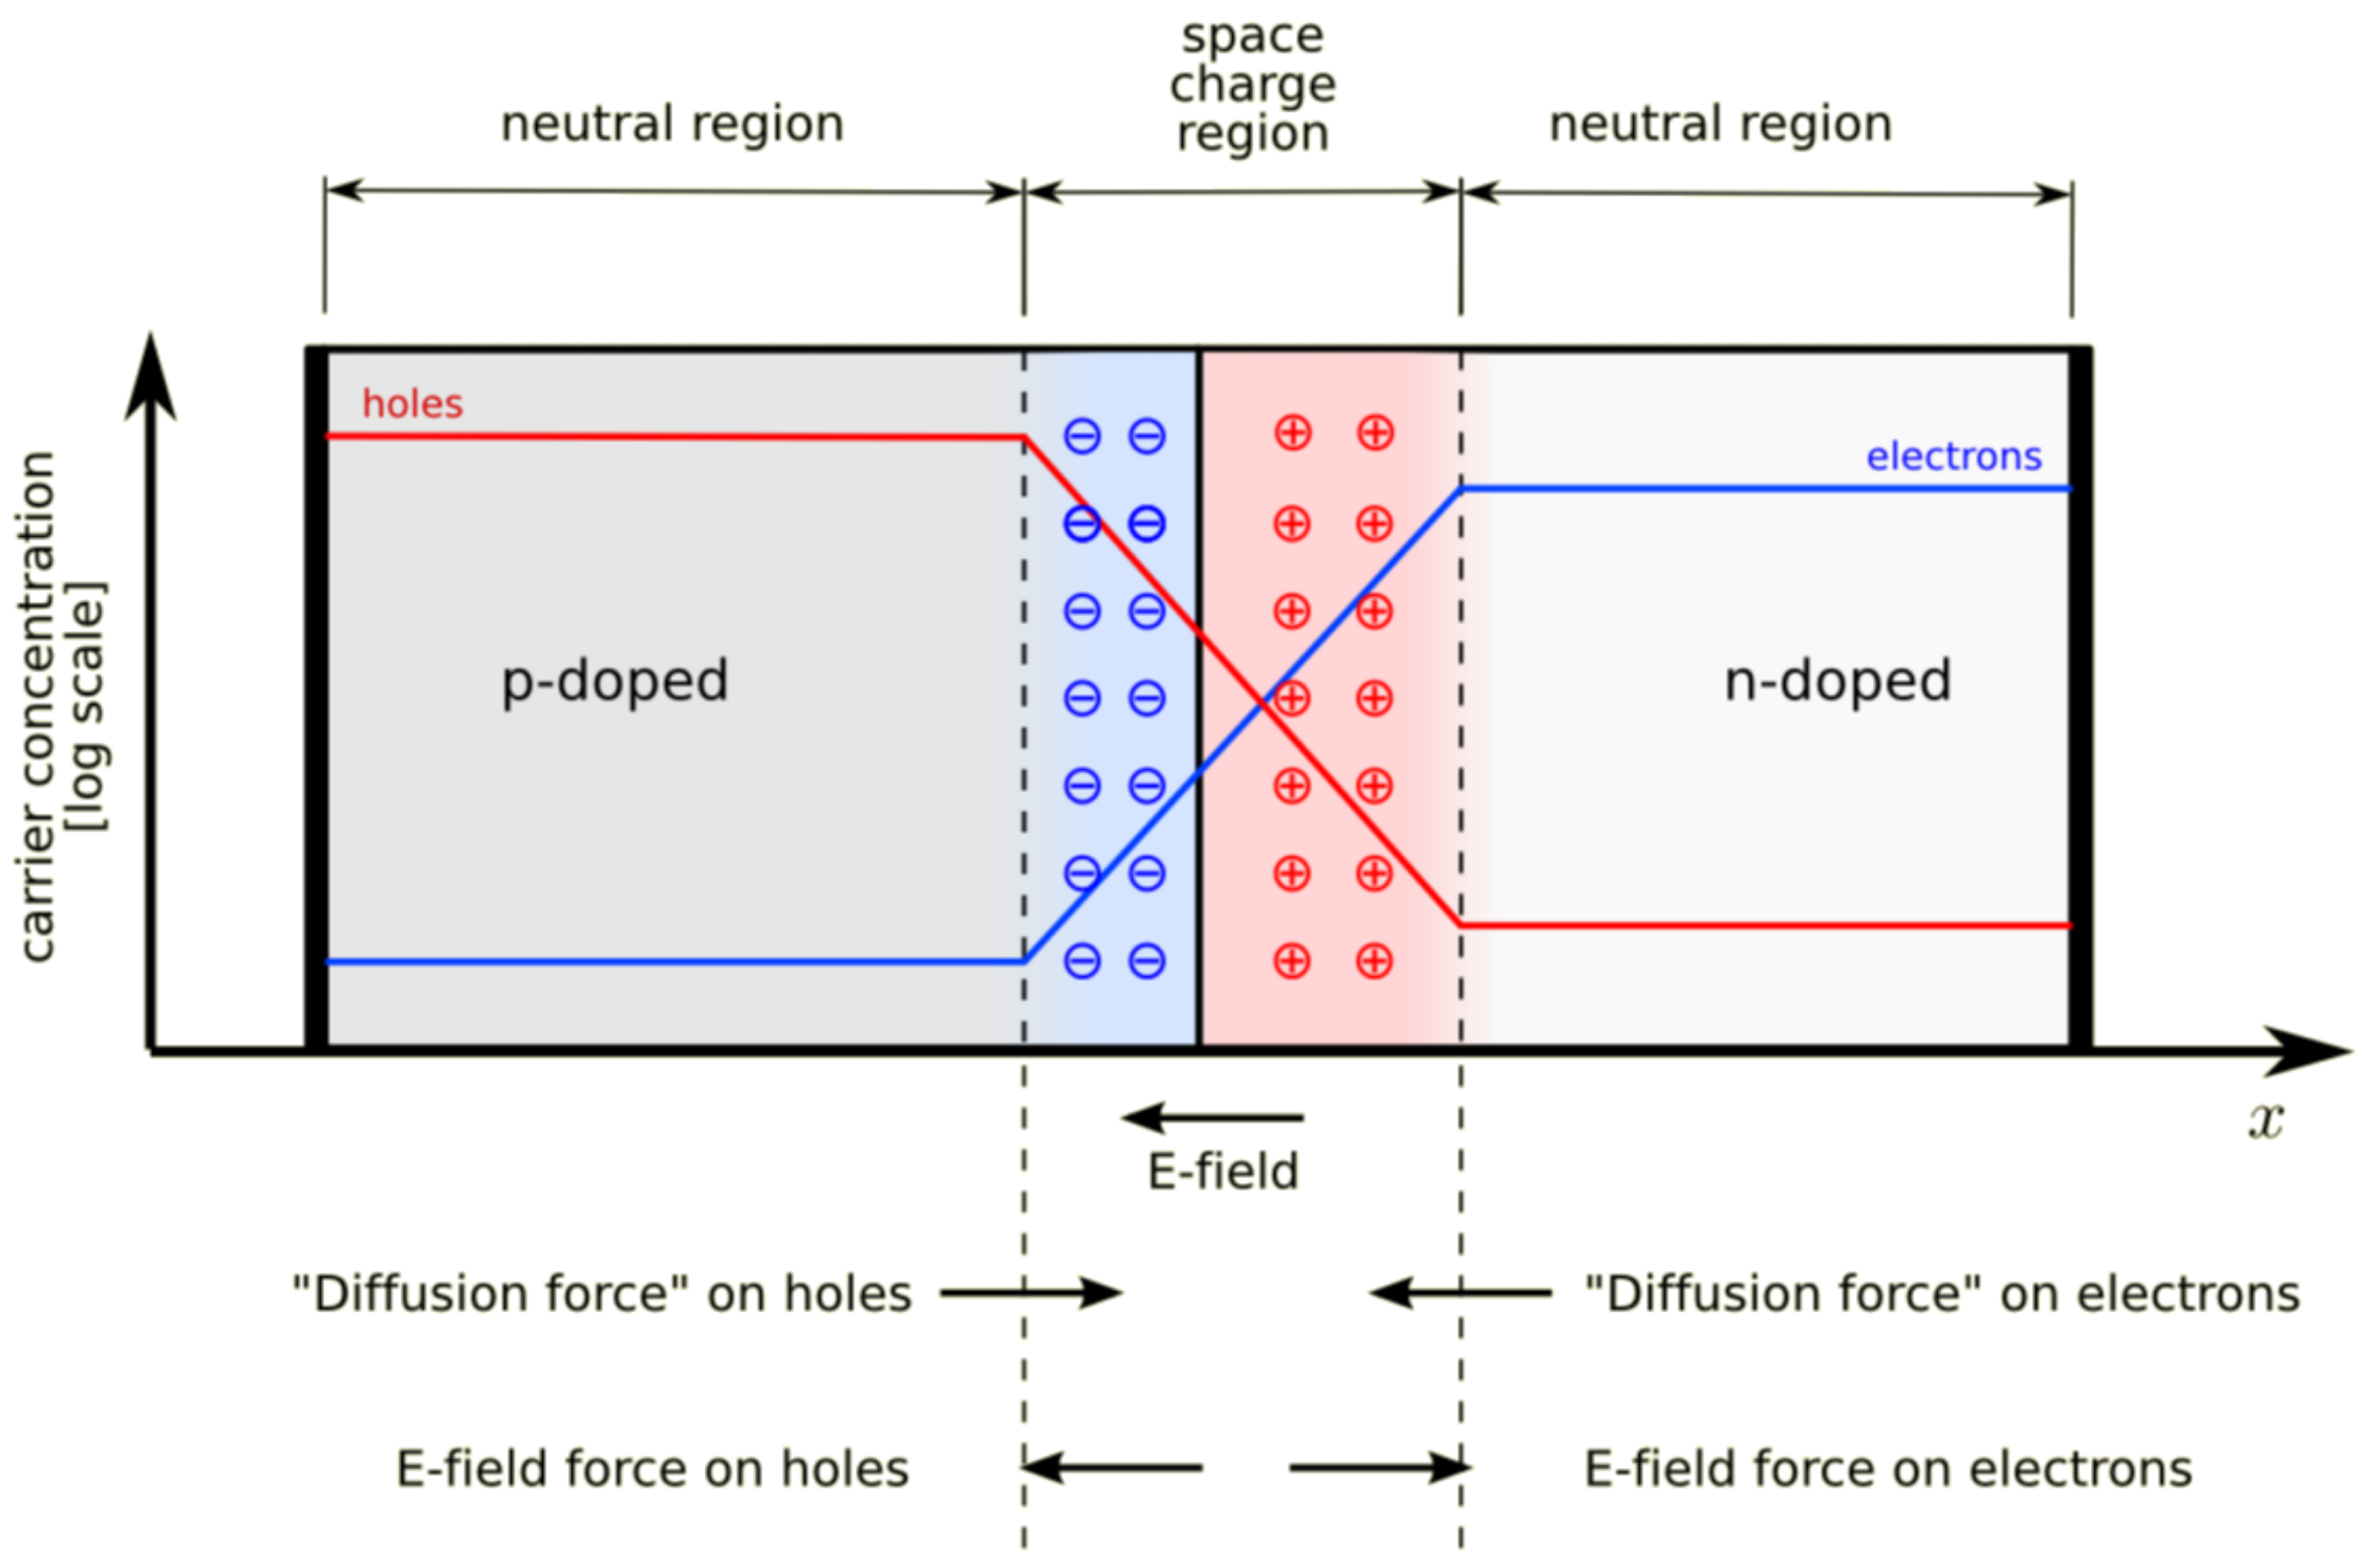
\includegraphics[width=1\textwidth]{pnfigur.png}
		\caption{ A pn-junction in equillibrium. Electron concentration is shown by the blue line, and correspondingly the red line for the holes. Red and blue zones indicate respectively positive and negatively charged regions, while grey is neutral. Forces and field directions are shown in the bottom of the figure. No bias voltage has been applied.
		By TheNoise at English Wikipedia, CC BY-SA 3.0, https://commons.wikimedia.org/w/index.php?curid=3833411.
		Accessed: December 13th 2021.
		}
		\label{fig:pnjunc}
	\end{figure}
	
	As the two regions are joined, electrons diffuse into the p-region and holes into the n-region leading to the recombination of electron-hole pairs as they meet. This gives rise to a region at the boundary, of immobile acceptors and donors, whose charge is not compensated by mobile charge carriers. We call this site the \textbf{depletion layer} \cite{solidstatephysicsbook}, see figure \ref{fig:pnjunc}. The thickness of this layer is around $0.1$ to $1 \mu$m \cite{solidstatephysicsbook}. An electric field arises due to the presence of the immobile ionized donors and acceptors. The electric field points from the net-positively charged n-region into the negatively charged p-region, presenting an obstacle for holes to move from the p-region to the n-region. The depletion layer widens, and the field strength increases, until an equilibrium between the electromagnetic and diffusion forces is reached. There is hence a \textbf{diffusion current} across the region for those carriers with enough energy to overcome the opposing electric field, and a \textbf{drift current} due to the presence of the same field \cite{solidstatephysicsbook}. The chemical potential in the p-doped region lies close to the VBM. In the n-doped region, it is close to the CBM \cite{solidstatephysicsbook} . However, if we apply a voltage across the depletion layer the equilibrium between these currents is broken such that a net current\cite{solidstatephysicsbook} is produced,
	\begin{equation}
		I = I_\text{diffusion} - I_\text{drift} = I_0\left(e^{eV/k_BT}-1\right),
	\end{equation}
	were $V$ is the so-called \textbf{bias voltage}. This bias voltage is essentially what lets the diode function as a valve for the current, and in our case allows for the build up of charge in the pixel.
	
	\subsection{The MOS capacitor as the pixel}
	The MOSCAP is a part of the so-called MOSFET structure. A MOSFET is a type of transistor\footnote{A transistor is an important basic building block, of modern electrical circuits, and acts as an amplifier or switch for the current.} made from the principle of the pn-junction and is usually constructed from silicon \cite{comphistmus}. A MOSCAP is constructed by forming a layer of silicon dioxide on top of a p-doped semiconductor. On top of this, a metal or polycrystalline silicon is deposited \cite{ccdwiki}, functioning as an electrode, also called the gate. This is the source of the bias voltage \cite{solidstatephysicsbook}. Silicon dioxide is a dielectric insulator, so this construction is akin to a planar capacitor. See figure \ref{fig:mosfet}.
	
	\begin{figure}[h!]
		\centering
		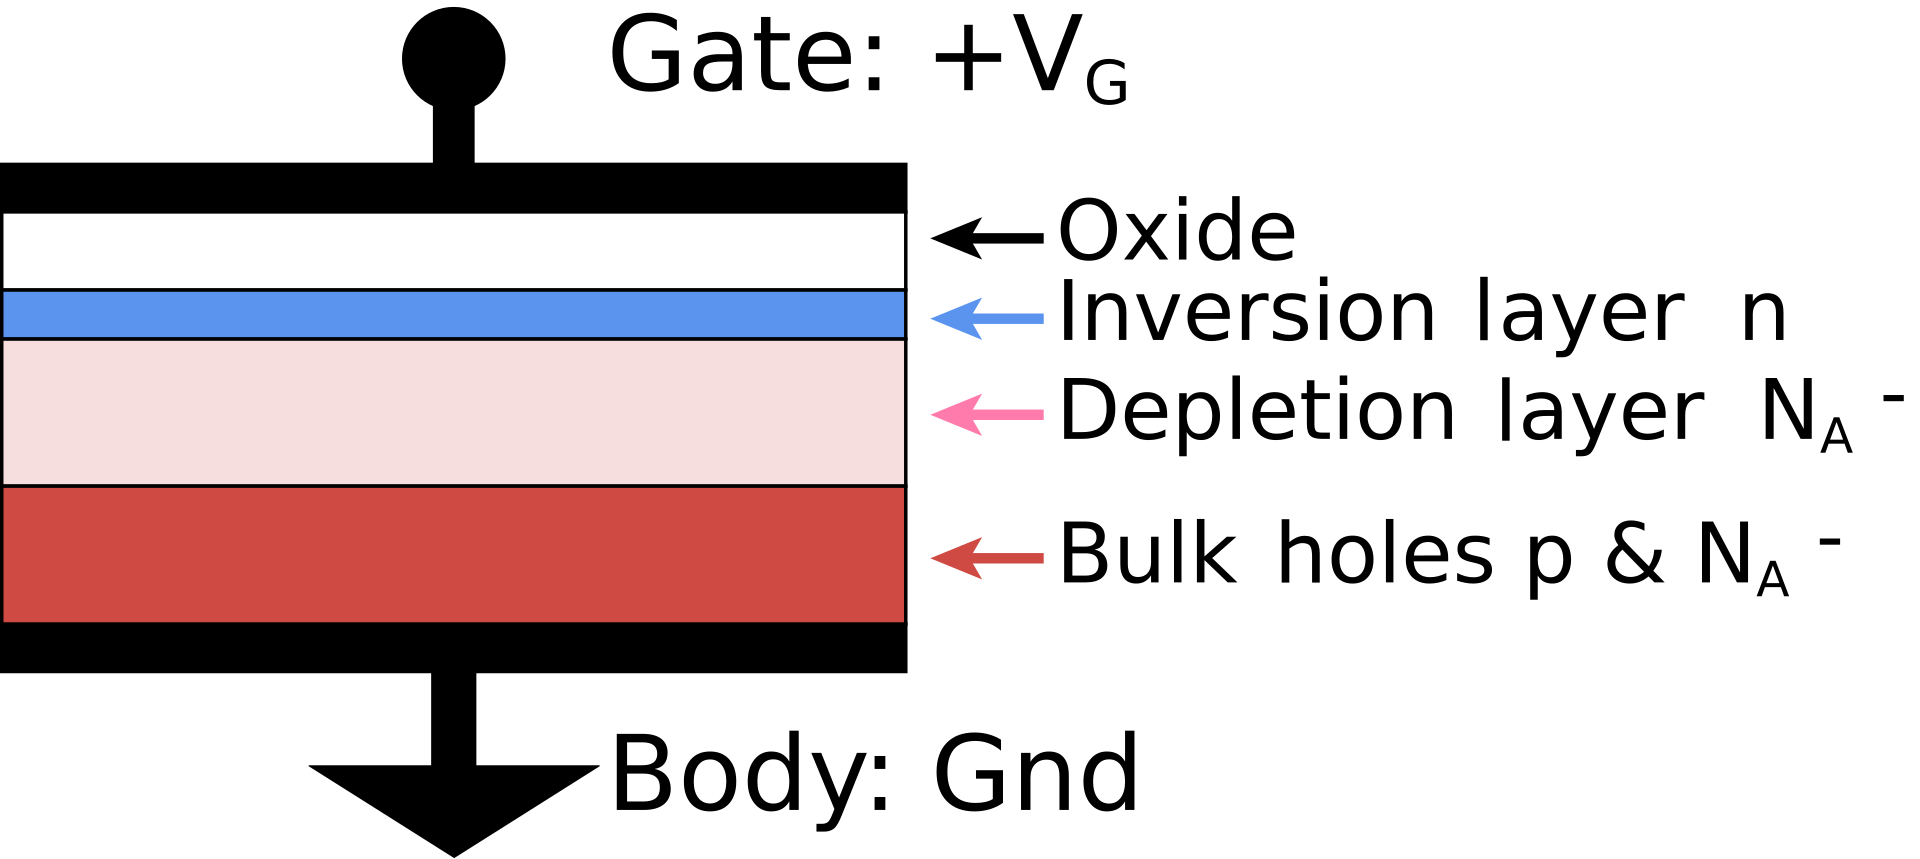
\includegraphics[width=0.5\textwidth]{MOS_Capacitor.png}
		\caption{A MOS capacitor (MOSCAP). Image by Brews ohare — Own work. Licensed under CC BY-SA 4.0, via Wikimedia Commons.
		}
		\label{fig:mosfet}
	\end{figure}
	When a voltage is applied to the gate, holes in the body, the p-type substrate, will be repelled, and minority electrons will be attracted, generating a depletion layer underneath the oxide layer. If the voltage is great enough, enough electrons will be attracted, and electrons become the majority carriers, forming an n-type region. We call this layer an \textbf{inversion layer}. The threshold voltage at which this happens is an important parameter. It is defined as that voltage, at which the density of the electrons in the inversion layer is the same as that of the density of holes in the p-type substrate \cite{solidstatephysicsbook}. 
	
	If in addition, two so-called \textbf{terminals} are included on either side of the body, consisting of n-doped regions (opposite type compared to the body type), the source, and the drain, we call the structure a \textbf{MOSFET}. In the case of a p-type (n-type) body, and two n-type (p-type) terminals, we denote it an nMOSFET (pMOSFET)  or n-channel MOSFET. This makes up two pn-junctions. As voltage is applied to the gate and the inversion layer forms, a channel is formed that will allow current flow. The higher the voltage the greater the electron carrier density, and hence the greater the current flow between the two terminals. Transistors either amplify or switch electronic signals, and are essential building blocks in electronics. 
	
	\subsection{CCD charge generation during exposure of the chip}
	We are now ready to describe charge generation in the CCD pixel. Before exposure of the CCD, the MOSCAPs in the array are biased into the depletion region \cite{CCDbook}, thus having not formed the inversion layer at this point. The gate is then biased positively (in n-channel MOSCAPS) above the threshold for inversion, creating an n-channel below the gate, just as in the MOSFET structure. In practice chips are constructed such that the gates are long wires spanning the length of the chip\cite{teledyneart}. In a single pixel usually 4 such wires (gates) are present. See figure \ref{fig:pixel} for an illustration of a real pixel. The CCD pixel structure, of which there are usually millions in a chip\cite{CCDdatareductionguide}. Charge collects in a buried channel\cite{teledyneart}, the region below the insulator. The insulator is present to keep charge away from the surface. Columns in the chip are separated by a channel stop\cite{teledyneart}. The gates are usually electrodes of polysillicon \cite{CCDbook}, since this material is transparent to incoming light above a wavelength of $400nm$.
	
	\begin{figure}[h!]
		\centering
		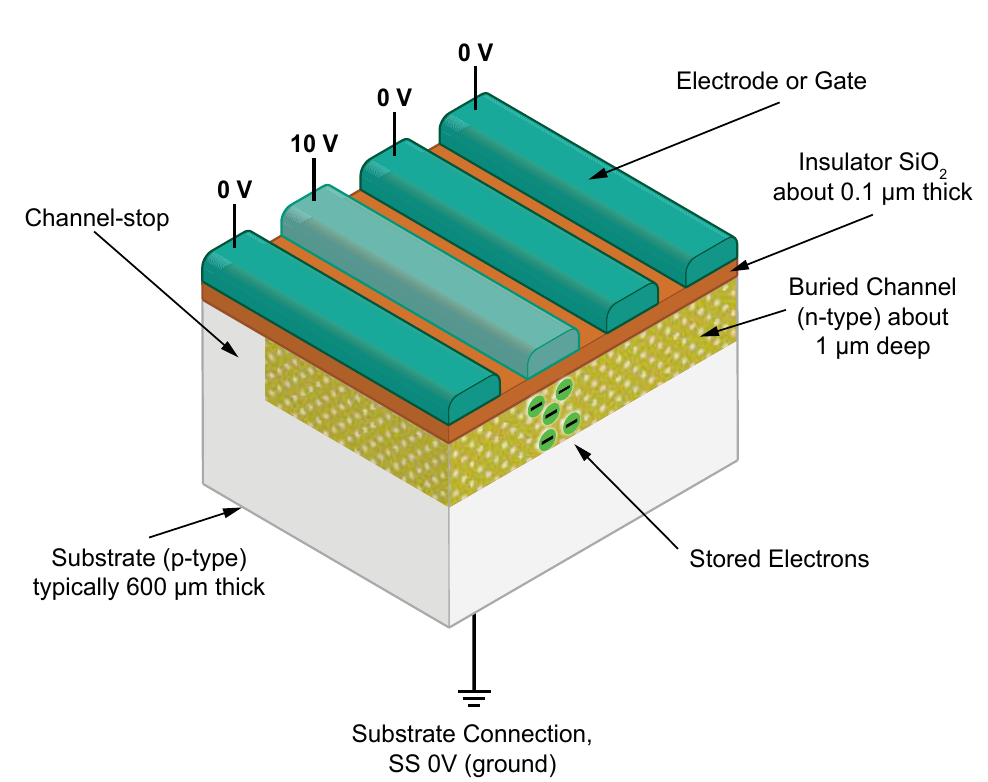
\includegraphics[width=0.95\textwidth]{pixel.png}
		\caption{The CCD pixel structure\cite{teledyneart}, of which there are usually millions in a chip\cite{teledyneart}. Charge collects in a buried channel, the region below the insulator. The insulator is present to keep charge away from the surface. Columns in the chip are separated by a channel stop\cite{teledyneart}. The gates are usually electrodes of polysillicon\cite{teledyneart}, since this material is transparent to incoming light above a wavelenght of $400nm$ \cite{teledyneart}. 
		}
		\label{fig:pixel}
	\end{figure}
	
	After the bias voltage is applied, holes are pushed far into the body substrate, and no mobile electrons remain; the CCD is in a non-equilibrium state called \textbf{deep depletion} \cite{CCDbook}. Now the chip is ready to detect photons, and formally the exposure begins. 
	
	As photons strike the depletion region, an electron-hole pair is formed and separated by the electric field. See figure \ref{fig:ccdsect}. Charge is hence accumulated just below the surface. This charge generation process can occur until a new thermal equilibrium is reached, a state which we call \textbf{full well}. The full well is a saturation effect, after which electrons may spill into neighboring pixels. The latter effect is called bleeding. This does not necessarily coincide with digital saturation, at which conversion of the signal from a current to a digital signal, in the analogue-to-digital converter, saturates due to lack of available bits. The latter form of saturation is studied in the characterization procedure below, since the Atik 414EX detector displayed this effect.
	
	Electron-hole pairs may also be created by thermal excitations anywhere in the array, generating noise referred to as dark current \cite{CCDdatareductionguide}. This effect is linear with time and follows a Poisson distribution\cite{CCDdatareductionguide} since they are rarely occurring stochastic incidents. Dark current may be corrected for and is a crucial part of the characterization procedure.  
	
	\subsection{CCD charge transfer and image readout}
	After the phase of charge generation, usually called \textbf{exposure} (or \textbf{integration}), the accumulated charge must be read and interpreted as a digital signal in the computer. This digital signal should ultimately result in a value in each pixel\cite{handbookofccdastronomy}. This is done by transferring the charge from the array, and sending the resulting electrical signal through an \textbf{analog-to-digital converter (ADC)} which will convert the analog signal of charges into a digitized signal that can be interpreted by a computer. This stage is called readout and happens on a line-by-line (row-by-row) basis \footnote{Here a line denotes a row in the CCD MOSCAP array} \cite{teledyneart}. Rows are shifted down one at a time until they reach the \textbf{readout register} (the final row). Within each row, each pixel is read out sequentially (horizontally), and transferred into the output amplifier. See figure \ref{fig:ccdreadout}. An overview of the detector may be seen in figure \ref{fig:ccdreadreg}.
	
	\begin{figure}[h!]
		\centering
		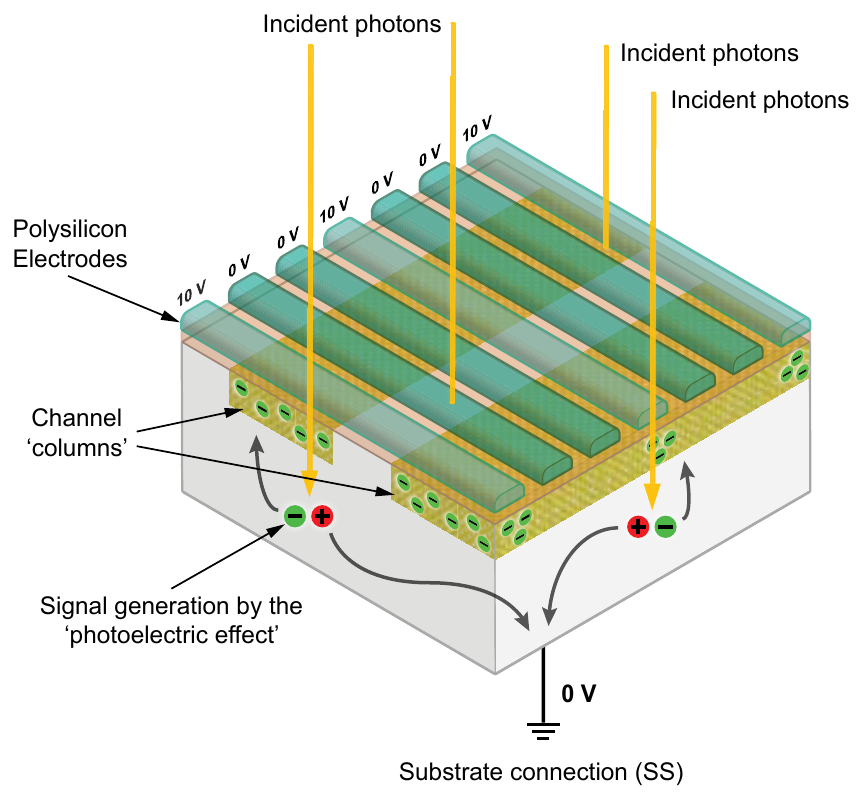
\includegraphics[width=0.95\textwidth]{ccdsect.png}
		\caption{A section of the CCD chip showing channels (columns) and electrodes \cite{teledyneart}. During exposure, incoming photons generate electron-hole pairs (in the figure referred to as "\textit{signal generation by the 'photoelectric effect'}") as described above, and charge accumulates in the channels. At readout, after an exposure has been completed, rows of charge is transferred downwards along the channel (along the columns). After a row of charge has been transferred out of the chip and into the readout register, the row is horizontally transferrred into the output amplifier. This operation is performed for every row of charge.
		}
		\label{fig:ccdsect}
	\end{figure}
	
	If the CCD chip is not shielded, then during readout, the chip is exposed to light, and hence the shifting process should be very fast, to avoid smear in the image. This however poses another problem, as a faster readout process results in a higher noise level \cite{handbookofccdastronomy, obsAstMichrichReadout}. This issue is solved in a \textbf{frame transfer CCD} by a shielded area of the chip, equal in size to the photosensitive area\cite{ccdwiki}. The shielded area typically consists of a highly reflective material, such as aluminum. After exposure, the rows are rapidly shifted into the shielded area, after which the necessary time to read out the measurements is available\cite{obsAstMichrichReadout}. A frame transfer CCD is depicted in figure \ref{fig:ccdframetransfer}. This can also be achieved via a \textbf{mechanical shutter}. 
	
	\begin{figure}
		\centering
		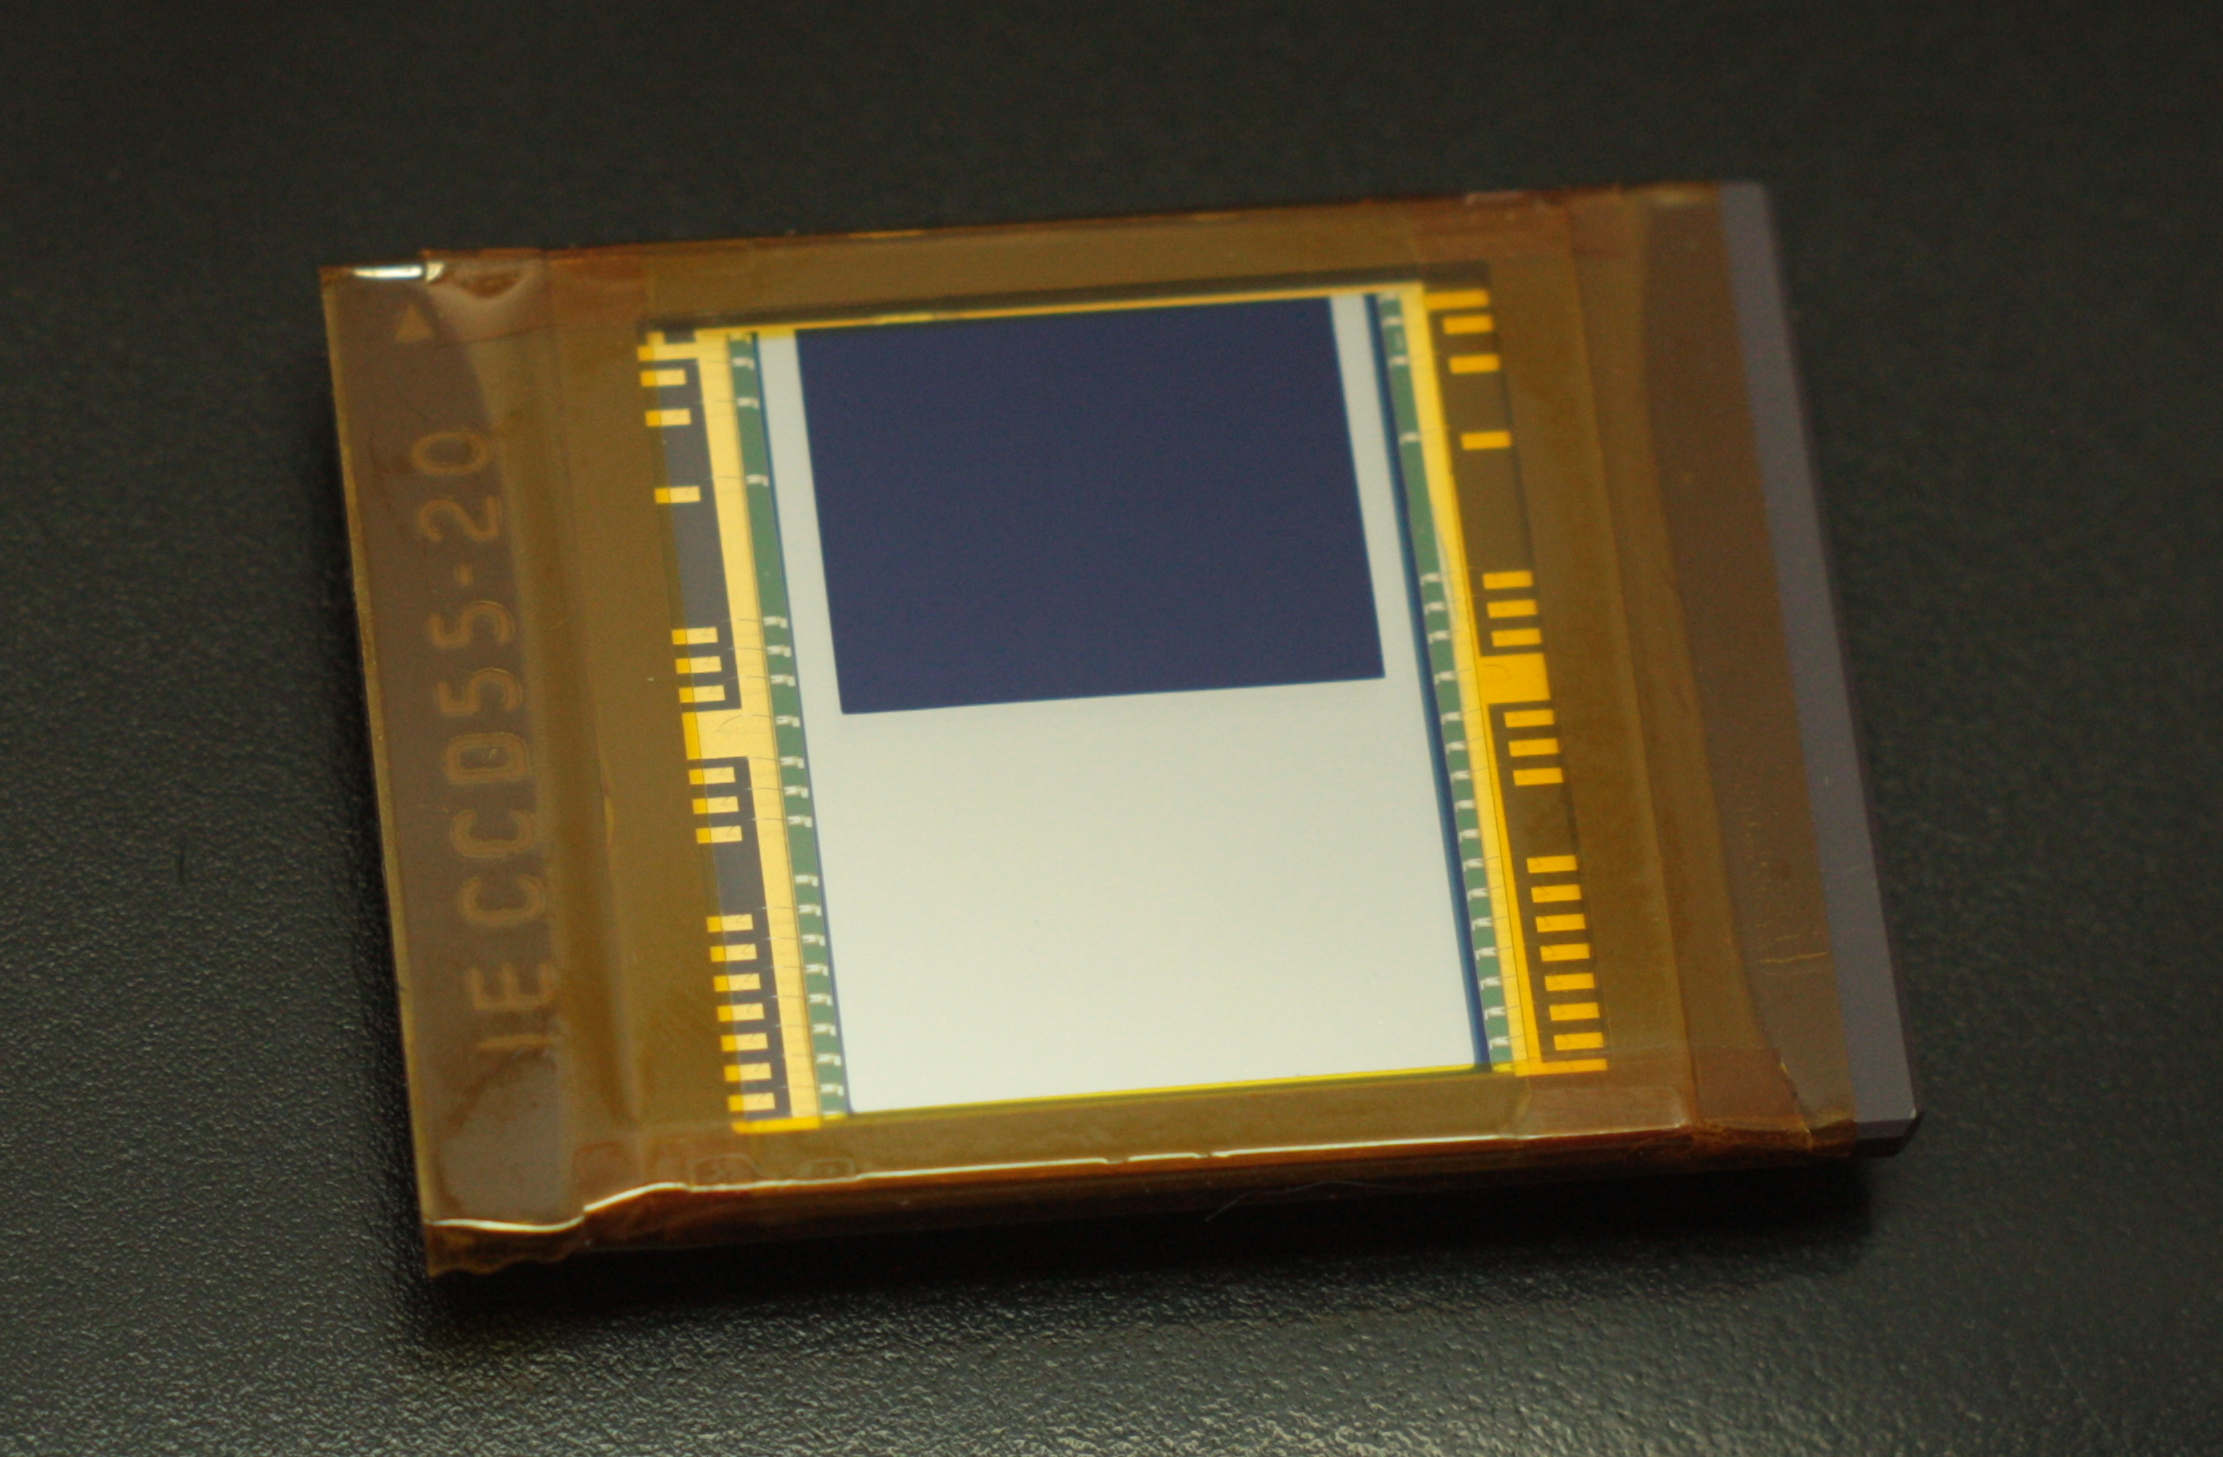
\includegraphics[width=1\textwidth]{frametransferccd.jpg}
		\caption{An e2v technologies CCD55-20, which is a frame transfer CCD sensor with $13$ mm $\times \;17.3$ mm image size and $576 \times 770$ pixel resolution. At the top, the photoactive region is seen, and at the bottom the aluminium shielding can be seen. Source: Olli Niemitalo, Wikipedia.} 
		\label{fig:ccdframetransfer}
	\end{figure}
	
	The detector used to develop the test procedure does not have a mechanical shutter, and we should hence characterize any potential time offset that may occur as a result of the extra exposure during readout.
	
	\begin{figure}
		\centering
		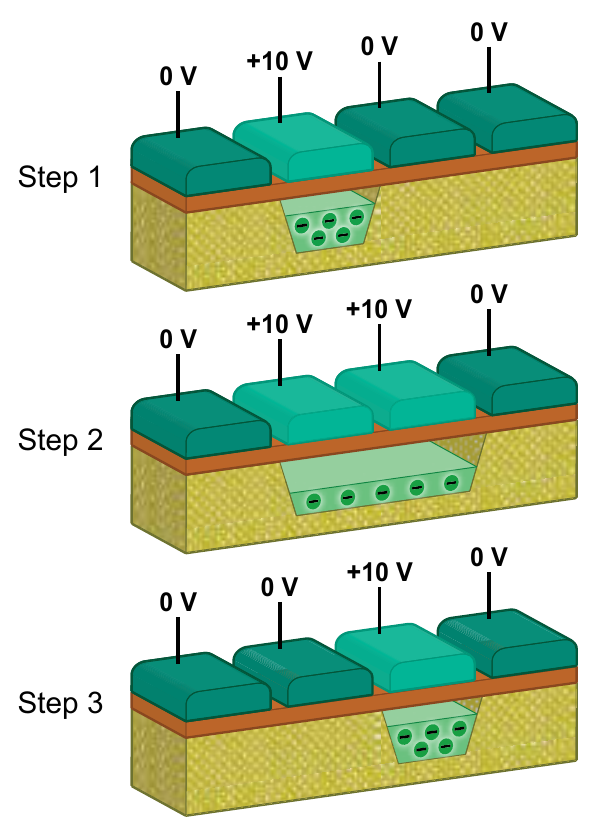
\includegraphics[width=0.5\textwidth]{readoutprinciple.png}
		\caption{An illustration of the charge readout principle of the CCD \cite{teledyneart}. Electrodes are alternately biased with high and low voltages to transfer the charge.
		} 
		\label{fig:ccdreadout}
	\end{figure}

	\subsection{Different kinds of CCDs}
	In this section, the different kinds of CCDs will be briefly discussed.
	
	\subsubsection{Back- and front illuminated CCDs}
	
	A CCD detector can be either \textbf{front illuminated} or \textbf{back illuminated}. The difference is in the direction from which photons arrive at the detector. In an ordinary CCD, which is front illuminated, photons are detected by illumination of the front of the detector. In this design, photons impinge from the same side as the gate electrodes. The electrodes may reflect or even absorb photons, which are then not detected. Hence the quantum effieciency will be lowered, and is usually around $50-60\%$\cite{backilluone}. Quantum efficiency is a measure of how many of the photons illuminating the surface of the detector are converted to electrons that are then measured. In a back illuminated CCD design, photons impinge from the back \cite{backillutwo}, via the bulk substrate. In this design quantum efficiencies are significantly higher, up to $95\%$\cite{backilluone} but the substrate will have to be thinned to allow photons to reach the photoactive region.
	
	
	%\subsubsection{CMOS sensors}
	%\textbf{Complementary metal–oxide–semiconductors} (CMOS) are like a CCD in the sense that they consist of an array of photoactive cells that, via the photoelectric effect, converts photons into electrons. They differ in the sense that, instead of transferring the induced charge across an array, to then read out the charge as a digital signal, the charge is converted to a voltage at the pixel site. This voltage is then transferred by circuitry and converted into a digital signal. This allows for readout during exposure of the CMOS. CMOS sensors are cheaper to produce, and have faster readout times. The disadvantage is lower sensitivity and higher noise levels. CMOS sensors are in general not used for Astronomical purposes due to the lower sensitivity, but are fast approaching the quality of CCDs. Because they are easier and cheaper to produce, they are readily used in most consumer products such as digital cameras. 
	
	\subsubsection{Electron-multiplying CCD}
	An \textbf{electron-multiplying CCD} (EM-CCD), is a CCD that is designed to perform at fast readout rates while offering a high degree of sensitivity\cite{EM-CCD}. In a traditional CCD, high sensitivity can be achieved, while the readout noise is kept low, if the CCD is read out slowly. Above, it was briefly mentioned that a higher readout speed results in a higher noise level. This is because a high readout speed requires a wide bandwidth of the charge amplifier\cite{EM-CCD}, but noise scales with the bandwidth of the amplifier. In an EM-CCD this is overcome by multiplying the charge signal, before the charge amplifier\cite{EM-CCD}. In this case the ratio of readout noise to signal can be made  small. In this way, readout noise can be effectively eliminated, and at high readout speeds.
	
	
	Now that a full description of CCD physics, and how a photosensitive detector works, has been presented, the basis of the testing procedure will be presented in the next section.
	
	\begin{figure}
		\centering
		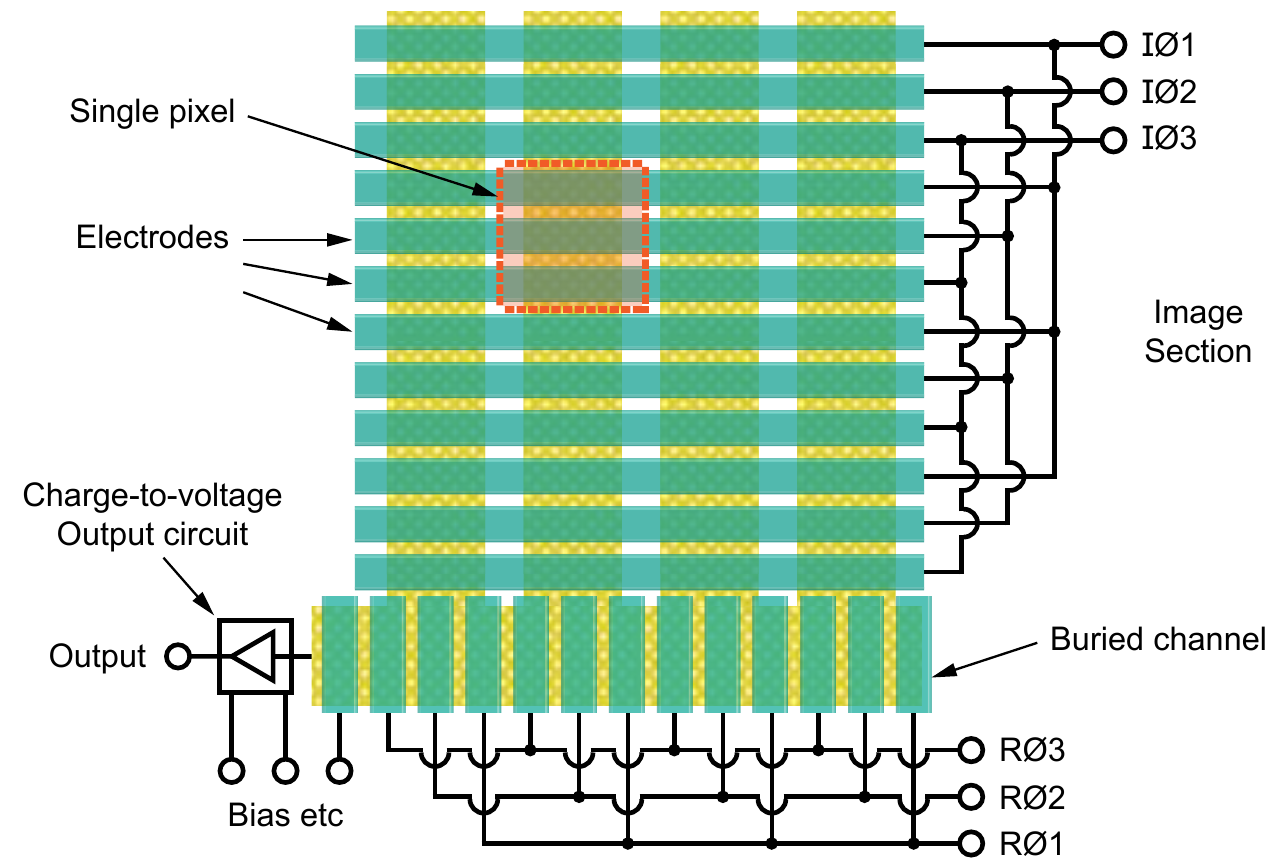
\includegraphics[width=0.95\textwidth]{readoutregister.png}
		\caption{An illustration of the CCD detector with readout register \cite{teledyneart}. A $4\times4$ image section (photoactive region, 16 pixels) is shown. Below the image section, the readout register is shown. The electrodes are oriented orthogonal to those of the image section, allowing for horizontal readout. One row is read out at a time, one pixel at a time, which is usually fed into an amplifier (not shown), before being fed into the \textbf{ADC} (analog to digital converter). The ADC converts the analog signal into a digital one, which the computer can interpret. The ADC has a "Charge-to-voltage output circuit" that converts the amplified singal into a voltage, that may then be interpreted as a digital signal. In the stage after the readout register, we may apply a bias voltage (to be explained below).
		} 
		\label{fig:ccdreadreg}
	\end{figure}
	
	\section{Characterization of CCDs}
	The central characterization metrics of a CCD detector will be outlined in the following section. At first, two useful definitions are in order.
	
	\begin{tcolorbox}[colframe = white, sharpish corners]
		\textbf{Master frames}
		\begin{quote}
			A master frame, is a frame that results from addition of many frames, in order to construct a mean frame. This reduces noise in the image, and increases statistical power.
		\end{quote}
	\end{tcolorbox}

	\begin{tcolorbox}[colframe = white, sharpish corners]
		\textbf{Dark frames}
		\begin{quote}
			A dark frame is an image acquired while the chip is not exposed to light. It is used to study noise effects in a CCD detector and to construct the master bias frame discussed below.
		\end{quote}
	\end{tcolorbox}
	
	\subsection{Bias}
	Noise is introduced when the CCD charge is read out. This noise is called readout noise, and will be explained in detail in section \ref{ron}. Readout noise follows a gaussian distribution centered on zero \cite{handbookofccdastronomy, CCDdatareductionguide}. If we consider an image acquired at an exposure time of (effectively\footnote{By effectively zero we mean, as short an exposure time, as is permitted by the detector at hand. For the the Atik 414EX detector the minimum exposure time is $0.001$s.}) zero seconds, because of noise there will be negative values in some of the pixels. To avoid negative counts in an image that consists entirely of noise, an offset voltage is applied to the CCD. This voltage offset level is called \textbf{bias}, and is necessary since negative signals cannot be correctly amplified in the amplifier stage \cite{handbookofccdastronomy, CCDdatareductionguide}.
	
	In general the bias does not vary with time \cite{CCDdatareductionguide}, but the frame will show some level of structure \cite{handbookofccdastronomy}. These structures can arise from the mechanical construction of the chip, if the chip consists of multiple separately constructed regions joined together, or be an effect introduced during the thinning process. The structures may also result from bad columns that may have a significantly higher offset than the rest of the chip \cite{CCDdatareductionguide}. 
	
	To study the bias level in the CCD, a dark frame with effectively zero exposure time may be acquired. A master bias frame may be constructed from multiple such frames, and this frame should be subtracted from other images when analyzing data, since it is an effect that is artificially introduced.
	
	\begin{figure}[h!]
		\centering
		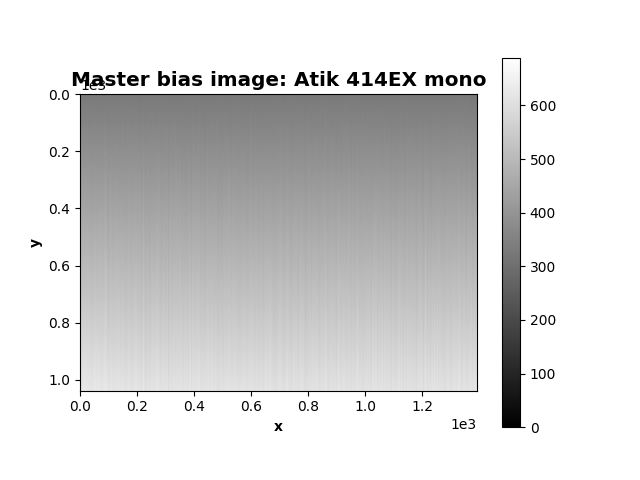
\includegraphics[width	=0.85\textwidth]{master_bias.png}
		\caption{A master bias frame was constructed by averaging over $300$ dark exposures of a flat field, with an exposure time of $0.001s$. The detector in question is an Atik 414EX detector. The frame exhibits some degree of structure. There are small streaks in the vertical direction, most noticeable on the left side of the image. There is also a slight gradient at the bottom of the image, which may be a dark current effect (see section \ref{sec:dc} for details) arising as the charge is read out row-wise from top to bottom. The bottom row of charge is the last to be read out. Dark current is strongly time-dependent and will be higher in those pixels.}
		\label{fig:masterbias}
	\end{figure}
	
	
	\subsection{Noise}
	For a CCD there are three main types of noise that must be characterized. These are \textbf{Readout noise (RON)}, \textbf{Photonic noise} and thermal noise, also called \textbf{dark current} \cite{handbookofccdastronomy}. They will each be discussed in turn below. 
	
	\subsubsection{Photonic noise and counting statistics}\label{sect:photonicnoise}
	Photon noise is the statistical fluctuation of the photonic flux detected by the CCD. Each photon is a discrete quantum, and the probability of the detection of the photon is independent of the other photons detected. This process follows a \textbf{poisson distribution} \cite{photonnoise}. \textbf{Poissonian statistics} is also called \textbf{counting statistics}. ADU count measurements are measurements of photons converted to electrons in the detector. Thus the relevant statistics for noise levels and image signals are of this nature.
	
	The poissonian distribution is given as\cite{observationelastronomi}
	\begin{equation}
		p(x) = \frac{n^x}{\mathrm{e}^n x!},
	\end{equation}
	where $n$ is the mean value of the distribution.
	\begin{equation}
		\langle x \rangle = \sum_{x=0}^\infty p(x) x = n.
	\end{equation}
	The standard deviation is\cite{observationelastronomi}
	\begin{equation}
		\sigma(x) = \sqrt{\sum_{x=0}^\infty p(x)(x-n)^2} = \sqrt{n}.
	\end{equation}
	We call this the \textbf{poisson noise}, which for electronics is usually called \textbf{shot noise}. The variance, $\sigma^2(x) = n$ is equal to the mean. The relative standard deviation, also known as the coefficient of variation, or the relative error, is given as 
	\begin{equation}
		\frac{\sigma(x)}{\sqrt{n}}= \frac{\sqrt{n}}{n} = \frac{1}{\sqrt{n}}.
	\end{equation}
	and is the \textbf{error in the measurement of $\sigma$}. That means, since we interpret $\sigma(x)$ as the noise in the distribution, that we may reduce the noise in the image, by increasing the number of events $N$. In this case an event is the measurement of a photon. The signal to noise ratio is the inverse of this moment\cite{SNRdef}
	\begin{equation}
		\textbf{SNR} = \frac{\text{Signal}}{\text{Noise}} = \sqrt{n}
	\end{equation}
	We may hence reduce photonic noise by observing bright objects that emit many photons, or by using longer exposure times. A more practical observation is that we may also mean over several acquisitions of the same image.
	
	A Poisson distribution tends to a normal (Gaussian) distribution for large numbers\cite{handbookofccdastronomy}. This is important since readout noise is Gaussian and follows the same statistics.
	
	\subsubsection{Readout noise}\label{ron}
	Readout noise is the stochastic process associated with the amplification of the signal \cite{handbookofccdastronomy}. It is introduced at the amplifier during the readout of the charge from the chip. It is usually quoted in terms of an RM number of electrons introduced per pixel upon readout \cite{handbookofccdastronomy}. Read noise cannot be eliminated, but it can be minimized. 
	
	There are two components to the phenomenon. The first one is an introduction of uncertainty at the ADC level. The process of converting the analog signal to a digital one is not perfectly repeatable but is a distribution of possible answers centered on a mean value \cite{handbookofccdastronomy}. The second component is extra electrons introduced by the electronics at work during readout.
	The size and temperature of the amplifier contribute to this noise. The temperature introduces as significant contribution due to thermal fluctuations \cite{handbookofccdastronomy}. 
		
	\begin{figure}[h!]
		\centering
		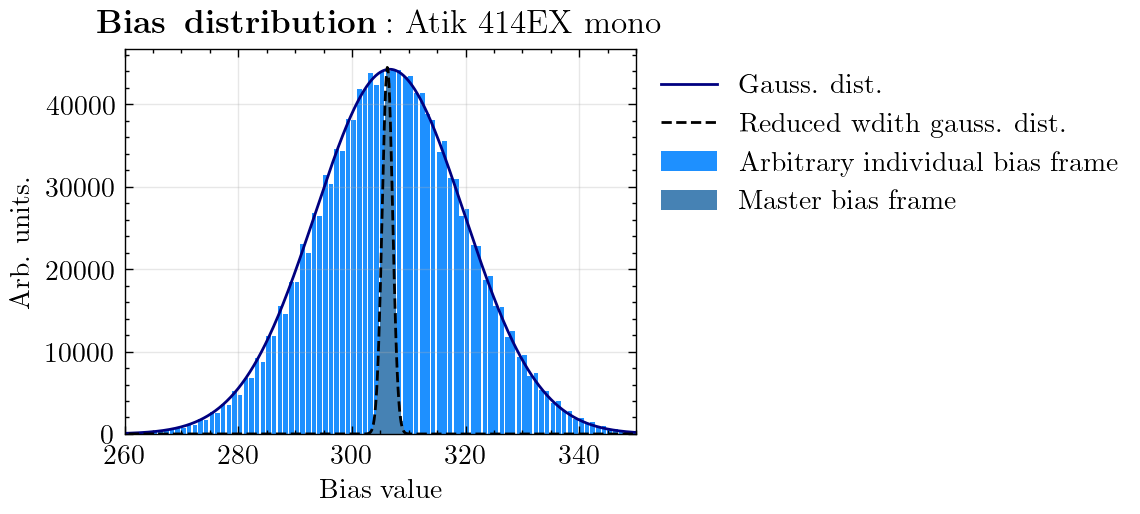
\includegraphics[width	=\textwidth]{gauss_bias.png}
		\caption{The bias distributions of an arbitrary bias frame, and that of the master bias frame, for the Atik 414EX detector. The width of the distribution is much smaller for the master bias frame, indicating a noise reduction. The individual bias frame displays a Gaussian behavior. The distribution in question is that of the entire chip, as the bias distribution for the Atik 414EX detector is very flat. This can be seen in figure \ref{fig:masterbias}.}
		\label{fig:rongauss}
	\end{figure} 
	
	Readout noise follows a Gaussian distribution. The width of this distribution, is the read noise (in electrons) divided by the gain (in electrons per count, see below for definition). This can be seen by producing a histogram of the values in the master bias frame. It is seen that this distribution is Gaussian with a mean value of the mean bias level offset, and a width corresponding to the readout noise. See figure \ref{fig:rongauss}. This is true under the assumption that the bias frame is flat, and shows no structure. This is seldom true globally \cite{handbookofccdastronomy}, but often a good assumption locally. 
	
	There are two ways we may compute readout noise. In the case of a flat detector, such as the Atik 414EX detector, we may acquire a series of $N$ bias frames. From these a master bias frame is constructed. From each of the individual frames in the data series, subtract this master bias frame. This corresponds to moving the gaussian distribution to a mean centered around zero, as we are subtracting the mean from the distribution. The resulting distribution, or frame, is noise with mean zero. The \textbf{standard deviation of this distribution is the readout noise}. Computing this value for all frames and meaning over the data series, results in a reduction in the error of the measurement of the readout noise by a factor of $1/\sqrt{N}$ (an improvement of the SNR by a factor of $\sqrt{N}$), as we are dealing with counting statistics\footnote{This is true because a poissonian distribution tends to a gaussian distribution in the limit of $N\rightarrow\infty$. Hence the same statistics apply.} (see section \ref{sect:photonicnoise}).
	
	If the detector is not flat, we may instead compute the readout noise levels from a \textbf{difference frame} \cite{obsAstMichrichReadout}. This is done by subtracting two bias frames, and interpreting the resulting image as the noise distribution. By subtracting two images we can effectively remove any non-flatness in the image, as any structure will be removed when subtracted \cite{obsAstMichrichReadout}, as it is a common factor. The standard deviation of the difference image, is the noise of the first, \textbf{and} the second image. Hence the noise (the standard deviation) increases by a factor of $\sqrt{2}$, which we should correct for as \cite{obsAstMichrichReadout}
	\begin{equation}
		\sigma_\text{single frame} = \frac{\sigma_\text{difference frame}}{\sqrt{2}} .
	\end{equation}
	The bias frame for the Atik 414EX detector (see figure \ref{fig:masterbias}), is relatively flat so the first method was used. 
	
	Generally, a slower readout rate will reduce the readout noise \cite{handbookofccdastronomy}. This poses another complication. A slower readout speed will introduce artifacts in the image in the form of streaks, if the chip in question does not have a mechanical shutter.  
	
	\subsubsection{Thermal noise and Dark current}\label{sec:dc}
	Thermal noise, also called \textbf{dark current}, is the current in the chip, resulting due to the thermal motion of the electrons in the solid-state material \cite{CCDdatareductionguide, handbookofccdastronomy}. Dark current may be studied in \textbf{dark-frames}, where no photo-electrons should be produced. The dark current depends linearly on time \cite{CCDdatareductionguide} and is usually given as electrons per second. We thus obtain the following relation for the dark current in the chip
	
	\begin{equation}\label{darkcurrenteq}
		\text{dark current} = \frac{\text{ADU} * \text{gain}}{\text{exposure time}},
	\end{equation}
	
	where the ADU value refers to the mean ADU / pixel in a dark frame, \textbf{after} the master bias frame has been subtracted from the image. Gain is described below in section \ref{sec:gain}.  
	\begin{figure}[h!]
		\centering
		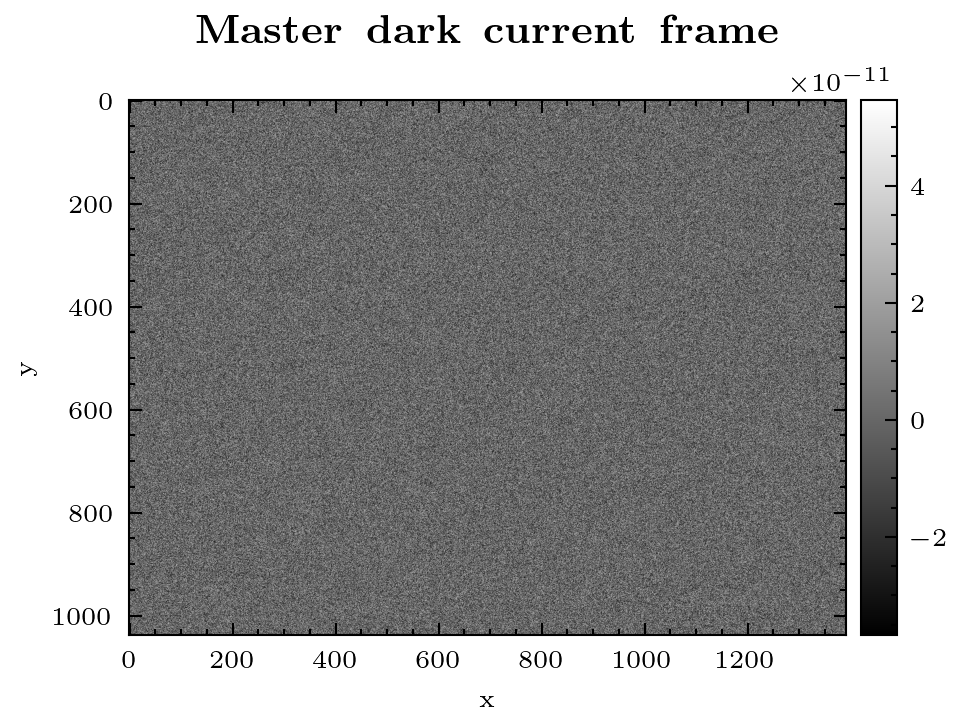
\includegraphics[width	=0.85\textwidth]{master_dark.png}
		\caption{A master dark current frame, for the Atik 414EX detector, constructed by averaging over many dark frames at a given exposure, subtracting the master bias frame, and then computing the dark current in each pixel according to equation \ref{darkcurrenteq}.}
		\label{fig:masterdarkcurrent}
	\end{figure}
	
	Thermal noise contaminates astronomical images making them hard to analyze and interpret. Fortunately, since dark current is strongly temperature-dependent, it can be practically eliminated by cooling the chip. The testing procedure should characterize the dark current levels as a function of temperature if possible. Readout noise levels are usually significantly greater than dark current levels \cite{handbookofccdastronomy}, so dark frames must be taken at long exposure times, to yield an appreciably large dark current effect that can be isolated from that of the readout noise \cite{handbookofccdastronomy}. This can also be achieved by averaging over a large number of dark frames, to average out readout noise. It should also be noted that a master bias frame should be subtracted from the dark fame to isolate dark current levels. 

	A master dark current frame can be constructed by averaging over many dark frames at a given exposure, subtracting the master bias frame, and then computing the dark current in each pixel according to equation \ref{darkcurrenteq}. Such a frame can be seen in \ref{fig:masterdarkcurrent}.
	
	\begin{figure}[h!]
		\centering
		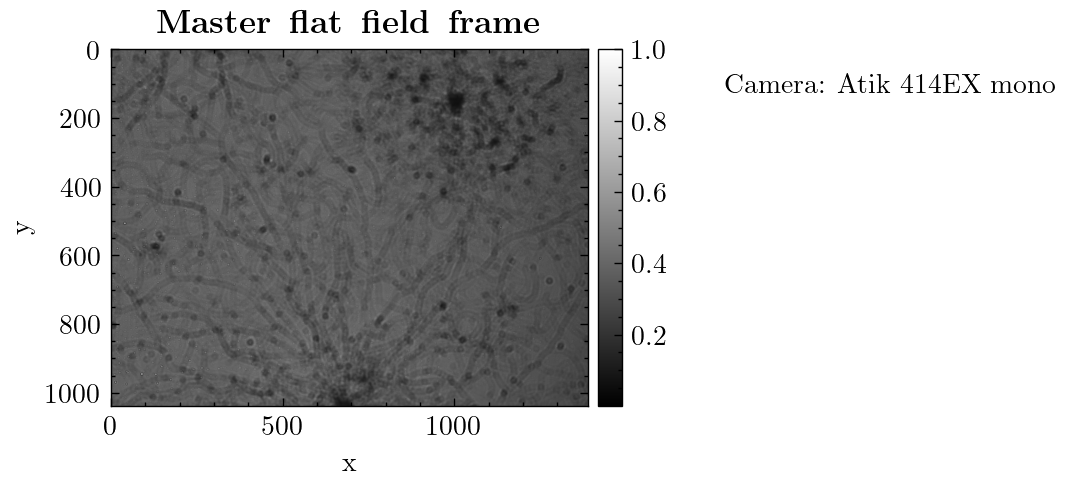
\includegraphics[width	=0.85\textwidth]{master_flat.png}
		\caption{A master flat frame that is constructed by averaging over $300$ light exposures of a flat field, with an exposure time of $10s$. After meaning, bias and dark current master frames are subtracted, and a hot pixel correction is applied. The resulting frame is then normalized as described in section \ref{sec:flat}. The non-flatness observed for this detector is probably not due to pixel-response-non-uniformities. It is most likely  due to dirt and grime on the detector window, perhaps from a fingerprint, causing obstruction of light and diffraction patterns to occur.}
		\label{fig:masterflat}
	\end{figure}
	\subsection{Flat fielding}\label{sec:flat}
	A CCD does in general not have a perfectly flat response to incoming light \cite{CCDdatareductionguide, handbookofccdastronomy}. By a flat CCD detector, we mean a detector that uniformly detects photons with the same efficiency and sensitivity across the entire photo-active region of the chip. 
	
	Some CCDs may be constructed by joining several photo-sensitive pieces of silicon or may be constructed by grinding off layers of a block of silicon to achieve a thin detector \cite{CCDdatareductionguide, handbookofccdastronomy, CCDbook, ccdwiki}. This grinding process may leave lines through the chip that can be either more or less sensitive to light. There may also be specks of dust or fingerprints on the detector window causing blocking of light and diffraction patterns in the image.
	
	To overcome this issue, we utilize flat-field frames. Such frames are acquired by imaging a flat field, such as a white flat screen. Any non-uniformities in the resulting image should be due to the non-flatness of the chip, or obstructing objects on the detector window. This flat field frame then represents the relative light sensitivity between pixels in the chip. Construction of a master flat-field frame can be used as a correction. This is accomplished by averaging over many flat exposures, and then normalizing the frame. Normalization is done by finding the mean pixel ADU-value in the array and dividing the rest of the pixels in the frame by this value. This should be done after a hot pixel correction that will be described below. This frame can now be used for flat field corrections. This is done by dividing an image in question with the master flat on a pixel-by-pixel basis. An example of such a master flat frame can be seen in figure \ref{fig:masterflat}.
	
	\subsection{Gain}\label{sec:gain}
	The relationship between the number of electrons generated at the chip, and the ADU value in the image, is called \textbf{gain}\cite{handbookofccdastronomy, CCDdatareductionguide}. The physical quantity measured by the CCD is the number of photons incident in the photoactive region, and \textit{not} the ADU signal. Photons, and in turn the electrons generated, are what obey Poissonian statistics. Thus, to understand the signal, and its noise levels, we need to be able to convert between ADUs and the number of generated electrons. 
	
	The gain value depends on the software used to read out the pixels and the detector electronics. When charge is read out from the chip, it passes through an amplification stage, charging a capacitor. The voltage from this capacitor passes through an \textbf{Analogue-to-digital converter (ADC)} which transforms the voltage signal into a string of binary digits. This conversion is done by the software, and the resulting units are \textbf{Analogue-to-digital units (ADUs)}\cite{handbookofccdastronomy}. At the ADC and software conversion levels we can scale the signal by an arbitrary factor while preserving the relative pixel values. This scaling factor is the gain \cite{handbookofccdastronomy, CCDdatareductionguide}. It can be expressed as
	\begin{equation}\label{gaindef}
		\text{gain} = g = \frac{\text{Number of electrons per pixel}}{\text{Number of counts per pixel}}
	\end{equation} 

	In each pixel there is a physical limit to the number of electrons that can be stored. This number is known as the \textbf{full well capacity} of the chip \cite{handbookofccdastronomy}. In addition, there is a maximum number that can be represented in the digitized signal. This depends on the number of digital bits  available to the ADC. For a $16$bit ADC, this number is $\text{ADU}_{\text{max, 16 bit}} = 2^{16} = 65563$. It is natural to choose the gain factor, such that the full well capacity, corresponds to the maximum digital value that we can store. This is not necessarily easy to achieve, as it is difficult to measure this parameter. If the full well capacity is such that after analog to digital conversion, the value cannot be stored digitally, that detector will display digital saturation. This happens because the digital signal saturates due to not having enough bits available to store the signal. This occurs for both the Atik 414EX detector, and the camera used to validate the test procedure.
	
	We can generally not assume the gain of the detector to remain constnat. Electric circuits change and deteriorate with time, and the amplification stage may change. We should measure the gain factor and compare it to the tabulated value provided by the manufacturer. It is also a good idea to measure the gain as a function of temperature in order to verify that it does not exhibit a strong temperature dependence.
	Gain can be measured by using subsequently acquired \textbf{flat field frames}. An expression for the gain factor that includes measurable quantities will be derived now, by exploiting the noise properties of the signal. We begin by noting that the noise in an image follows eq. (\ref{gaindef}). 
	\begin{equation}
		\text{Total noise in electrons} = \sigma_\text{total, $e^-$} = g * \sigma_\text{total, ADU} 
	\end{equation}
		
	The total noise in an image is comprised of several noise sources. They are independent, and the total noise squared is the sum of the squares contributing. We shall assume the detector to be cooled, and hence the main contributions to the noise are the photonic and readout noise. Thus we may write the total noise as
	\begin{align}\label{totalnoiselec}
		\sigma_\text{total, $e^-$}^2 = g^2\sigma_\text{total,ADU}^2 &= g^2\sigma_\text{photonic, ADU}^2 + g^2\sigma_\text{RON, ADU}^2
	\end{align}
	This relation lets us find an expression for the gain factor $g$, if we can measure the noise in the signal. 
	
	Consider two flat field frames taken subsequently, under identical conditions. We assume these two flat fields to be nearly identical. Let $\bm F_i^\text{unit}$ be the flux (mean counts per pixel if in ADU) in an arbitrary flat-field frame. The flux is measured in a unit (either ADU or electrons, $e⁻$). Any small changes in the incoming flux of light, perhaps due to the temporal drift in the intensity of the light source between the two acquisitions, can be corrected by multiplying the second frame by the ratio of the fluxes. This works under the assumption that a flux drift is linear between the two acquisitions. Small fluctuations between the two frames may now be attributed to noise. 
	
	The total noise in an arbitrary image is found by considering the difference image, where we have adjusted the latter flat field image for any changes in the flux. Such a frame must consist entirely of noise. The variance of this frame is
	\begin{align}
		\sigma\left(\bm F_1^{e^-} - \bm F_2^{e^-}\frac{\langle \bm F_2^{e^-}\rangle }{\langle \bm F_1^{e^-}\rangle }\right)^2 &= \text{Var}\left(\bm F_1^{e^-} - \bm F_2^{e^-}\frac{\langle \bm F_2^{e^-}\rangle }{\langle \bm F_1^{e^-}\rangle }\right) = \text{Var}\left(\bm F_1^{e^-}\right) + \text{Var}\left(\bm F_2^{e^-}\frac{\langle \bm F_2^{e^-}\rangle }{\langle \bm F_1^{e^-}\rangle }\right)\\
		\intertext{Where the last equality is due to the variance of the difference between two independent (uncorrelated) random variables is $\text{Var}(X-Y) = \text{Var}(X) + \text{Var}(Y)$. The variance of the difference image is twice that of the variance in an individual image. This is due to the additive nature of the variance (and having corrected for flux drifts in the second frame). Thus the total noise in an individual frame must be half this value}
		\sigma_\text{total,  $e^-$}^2 &= \frac12\sigma\left(\bm F_1^{e^-} - \bm F_2^{e^-}\frac{\langle \bm F_2^{e^-}\rangle }{\langle \bm F_1^{e^-}\rangle }\right)^2\\ &= \frac12\sigma\left(g\bm F_1^\text{ADU} - g \bm F_2^\text{ADU}\frac{\langle \bm F_2^\text{ADU}\rangle }{\langle \bm F_1^\text{ADU}\rangle }\right)^2\\
		&= \frac{g^2}{2}\sigma\left(\bm F_1^\text{ADU} - \bm F_2^\text{ADU}\frac{\langle \bm F_2^\text{ADU}\rangle }{\langle \bm F_1^\text{ADU}\rangle }\right)^2
	\end{align}
	which is the left-hand side of eq. (\ref{totalnoiselec}). On the right-hand side of the equation, the readout noise in electrons $\sigma_\text{RON, ADU}^2$, is estimated as outlined above in section \ref{ron}. The photonic noise contribution, $\sigma_\text{photonic, ADU}^2$ follows Poissonian statistics and is simply the mean of the detections in the two frames.
	\begin{align}
		\sigma_\text{photonic, ADU}^2 &= \frac12\left( \bm F_{1}^{e^-} + \bm F_{2}^{e^-} \right) = \frac{g}{2} \left(\bm F_{1}^\text{ADU} + \bm F_{2}^\text{ADU}\right)
	\end{align}
	By reinserting in eq. (\ref{totalnoiselec}), and isolating the gain factor, we obtain
	\begin{align}\label{eq:gainfactorest}
		g &=  \frac{\bm F_{1}^\text{ADU} + \bm F_{2}^\text{ADU} }{\sigma^2 \left(\bm F_1^\text{ADU} - \bm F_2^\text{ADU}\frac{\langle \bm F_2\rangle }{\langle \bm F_1\rangle }\right) - 2\sigma_\text{RON, ADU}^2}
	\end{align}
	
%	\begin{align}
%		\text{gain} = \frac{\bm F_1^\text{ADU} + \bm F_2^\text{ADU}}{\sigma^2 \left(\bm F_1^\text{ADU} - \bm F_2^\text{ADU}\frac{\langle \bm F_2\rangle }{\langle \bm F_1\rangle }\right) - 2\sigma^2_\text{RON}^\text{, ADU}}
%	\end{align} 
	 As an example, for the Atik 414EX detector, the gain factor is tabulated to be $\text{gain}_\text{tabulated} = 0.28 e^-\text{ADU}$\cite{atik414specs}. 
	 
	 It was measured to be $\text{gain}_\text{measured} = 0.24384\pm 0.000005 e^-/\text{ADU}$ (see table \ref{table:results}).
	
	\subsection{Hot pixels}
	A hot pixel is a pixel which has an ADU value that is significantly greater than the mean value in the image\cite{CCDdatareductionguide}. These should be corrected for. Such an effect can occur either because that pixel has a higher sensitivity to incoming photons, or because the dark current in that pixel is higher and/or not proportional to time in a linear way\cite{CCDdatareductionguide}. 
	A correction is achieved by constructing a mask of pixels which must be treated differently in the analysis of the data \cite{CCDdatareductionguide}.
	
	\subsection{Linearity}\label{sec:linearity}
	Linearity is the measure of the detectors response to changes in the flux of light incident on the detector. It is the relationship between the number ADUs in the image, and the number of incident photons. In other words, if one doubles the exposure time, or if the flux of the light source is doubled, we expect to have double the number of photons incident on the detector, and hence double the number of ADU counts in the image. 
	
	We may study this effect by acquiring frames at different exposure times, or different intensities of the light source, and comparing the mean ADU/pixel across exposure times. A detector is seldom perfectly linear, and the nonlinearity must therefore be characterized. This is crucial for astronomical purposes as was outlined in the introduction above.
	
	The nonlinearity of the detector may be defined as the deviation of a given measurement from the perfect linear behavior.
	
\end{document}